Wir betrachten als erstes Voronoi Kanten zwischen Punkt $P$ und Strecke $s$, diese bestehen grundsätzlich aus 3 Abschnitten. (i) und (iii) sind Strecken bzw. Strahlen. Es ist die Voronoi Kante zwischen dem Punkt $P$ und dem linken $A$ bzw. rechten Streckenende $B$. (ii) ist eine Parabel, deren Form ist abhängig vom Abstand zwischen $P$ und $s$. In welchem Abschnitt $P$ liegt ist egal, denn die Zusammensetzung der Voronoi Kante bleibt gleich.

\begin{figure}[h]
\begin{center}
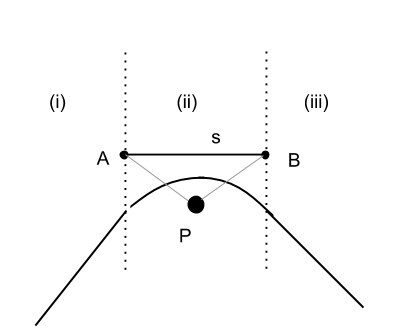
\includegraphics[width=7cm]{img/punkt-strecke.png}
\end{center}
\caption{Bisektor Punkt und Strecke}
\label{fig:c1}
\end{figure}

Betrachten wir nun die Bisektoren von zwei Strecken $s$ und $t$, dabei unterscheiden wir in (a) parallele Strecken und (b) nicht parallele Strecken.

\paragraph*{(a): parallele Strecken:}

\begin{itemize}
\item (1) $s$ und $t$ liegen auf einer Geraden (Spezialfall)
\item (2) überschneiden sich nicht
\item (3) überschneiden sich zum Teil oder ganz
\end{itemize}

Im Fall (2) und (3) entstehen 5 Bereiche:\\
(i) Gerade: Bisektor von den linkesten Punkten $A$ und $C$\\
(ii) Parabel: $s$ und $C$\\
(iii) Gerade: Gerade dazwischen\\
(iv) Parabel: $t$ und $B$\\
(v) Gerade: Bisektor von den rechtesten Punkten $B$ und $D$\\

\begin{figure}[h]
\begin{center}
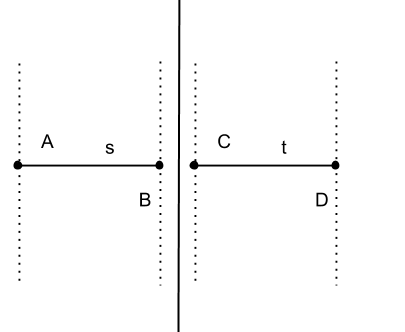
\includegraphics[width=7cm]{img/ssp1.png}
\end{center}
\caption{(1) Bisektor von zwei parallelen Geraden, auf einer Geraden.}
\label{fig:a1}
\end{figure}

\begin{figure}[h]
\begin{center}
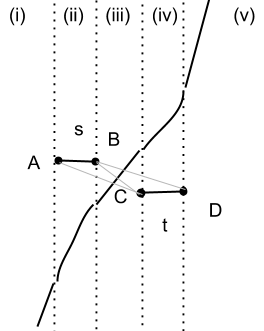
\includegraphics[width=7cm]{img/ssp2.png}
\end{center}
\caption{(2) Bisektor von zwei parallelen Geraden, keine Überschneidung.}
\label{fig:a2}
\end{figure}

\begin{figure}[h]
\begin{center}
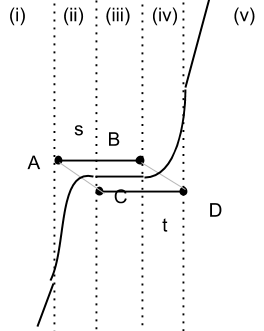
\includegraphics[width=7cm]{img/ss3.png}
\end{center}
\caption{(3) Bisektor von zwei parallelen Geraden, Überschneidung.}
\label{fig:a3}
\end{figure}

\begin{figure}[h]
\begin{center}
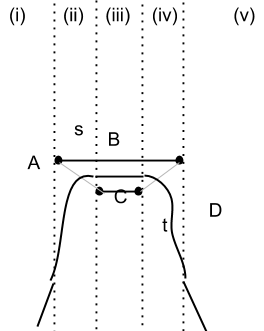
\includegraphics[width=7cm]{img/ss4.png}
\end{center}
\caption{(3) Bisektor von zwei parallelen Geraden, komplett innerhalb.}
\label{fig:a4}
\end{figure}

\paragraph*{(b): nicht parallele Strecken}

\begin{itemize}
\item (1) überschneiden sich nicht
\item (2) überschneiden sich zum Teil oder ganz
\end{itemize}

Hier entstehen im Fall (1) 4 Bereiche, im Falls (2) 7 Bereiche:\\

Erster Fall: wenn sie sich nicht überschneiden:\\
(i) Gerade\\
(ii) Winkelhalbierende\\
(iii) Parabel\\
(iv) Gerade\\

\begin{figure}[h]
\begin{center}
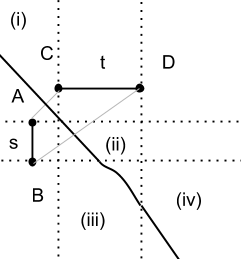
\includegraphics[width=7cm]{img/ssnpout.png}
\end{center}
\caption{(3) Bisektor von zwei nicht parallelen Geraden, keine Überschneidung.}
\label{fig:a5}
\end{figure}

Zweiter Fall: wenn sie sich überschneiden:\\
(i) Parabel\\
(ii) 2$\times$Winkelhalbierende\\
(iii) und (iv) Parabel\\
(v) Gerade\\
(vi) Parabel\\
(vii) Gerade\\

\begin{figure}[h]
\begin{center}
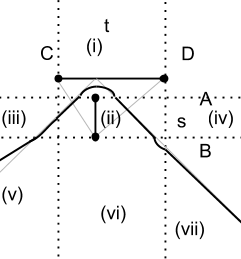
\includegraphics[width=7cm]{img/ssnpin.png}
\end{center}
\caption{(3) Bisektor von zwei nicht parallelen Geraden, mit Überschneidung.}
\label{fig:a5}
\end{figure}


Anzahl der Ecken: vielleicht wenn ich die Ecken weiß dann kommt man auch auf die Kanten.\\
Anzahl der Kanten: hm das weiß ich nicht.\\
Anzahl der Zellen: ist gleich Anzahl der Strecken.\\

Ich würde so wie bei den normalen Voronoi Diagrammen schauen was für Knoten es gibt und was die für einen maximalen Grad haben können und dann kann man das sicherlich irgendwie ausrechnen und die Kanten ergeben sich dann automatisch aus dem Gesamtdegree des Graphen oder so.


* Wie sehen die Voronoi-Kanten aus $\rightarrow$ Bilder von allen Fällen\\
* Aus wie vielen Ecken, Kanten und Zellen kann $VD(S)$ höchstens bestehen?\\
* Zeigen Sie dazu, dass die Voronoi-Regionen zusammenhängend sind.